%!TeX root = Thesis_LP.tex
\chapter{Introduction}
\setlength{\parindent}{0cm}
\setlength{\parskip}{1em}
Selon le dernier rapport du Groupe d'experts intergouvernemental sur l’évolution
du climat (GIEC), le réchauffement climatique est indiscutable et
trouve son origine dans l'activité humaine \citep{IPCC2014}. L’atmosphère et les
océans se sont
réchauffés, les quantités de neige et de glace ont diminué et les niveaux des
océans ont augmenté. \\
À partir de l'ère préindustrielle, les émissions des gaz à effet de serre (GES)
ont augmenté principalement à cause de l'industrialisation et de l'augmentation
de la population. Ceci a mené à l'accélération sans précédent de l'augmentation
des
concentrations atmosphériques de dioxyde de carbone de méthane et de protoxyde
d'azote (voir \Cref{fig:GES}).
Il faut s'attendre à ce que la poursuite des émissions de GES aggrave encore la
hausse des températures et provoque de nouveaux changements.
\section{Le problème du charbon}
La concentration du \ce{CO2} dans l’atmosphère varie de façon naturelle. La
\cref{fig:CO2} montre la variation des concentrations de \ce{CO2} dans les
derniers \num{650000} ans \citep{Epica,Siple,Vostok,WMO14}. Ces données montrent
une
concentration stable de
\ce{CO2} d'environ \SI{280}{ppm}, qui correspond à la concentration à la fin de
la dernière glaciation (\num{\pm 10000}). L'augmentation du \ce{CO2} au-dessus
de \SI{280}{ppm}
coïncide avec la révolution industrielle (autour des années 1800) et elle a
accéléré sans cesse jusqu'à nos jours pour atteindre la valeur d'environ
\SI{400}{ppm} en \num{2014}.
\begin{figure}[ht]
        \centering
        \begin{subfigure}[b]{.77\textwidth}
                \caption{Concentrations atmosphériques du \ce{CO2}, \ce{N2O} et
du \ce{CH4}.}
                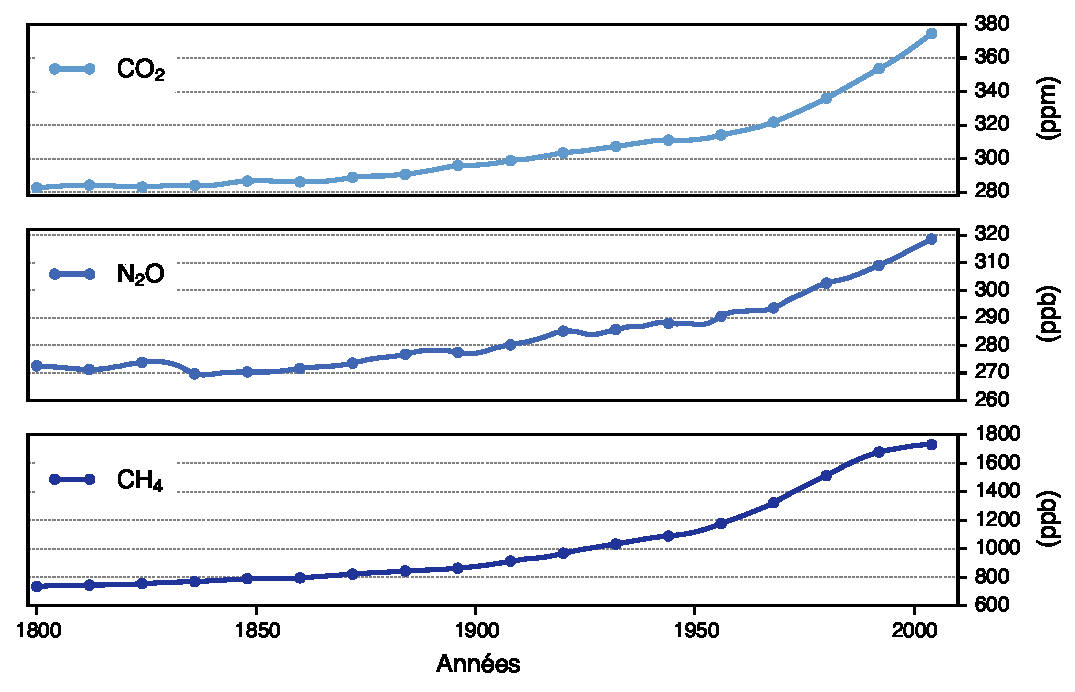
\includegraphics[width=\textwidth]{fig/GES.pdf}
                \label{fig:GES}
        \end{subfigure}%

        \begin{subfigure}[b]{.77\textwidth}
        		\caption{Concentration de \ce{CO2} dans l'atmosphère dans les
dernières \num{650000} années.}
                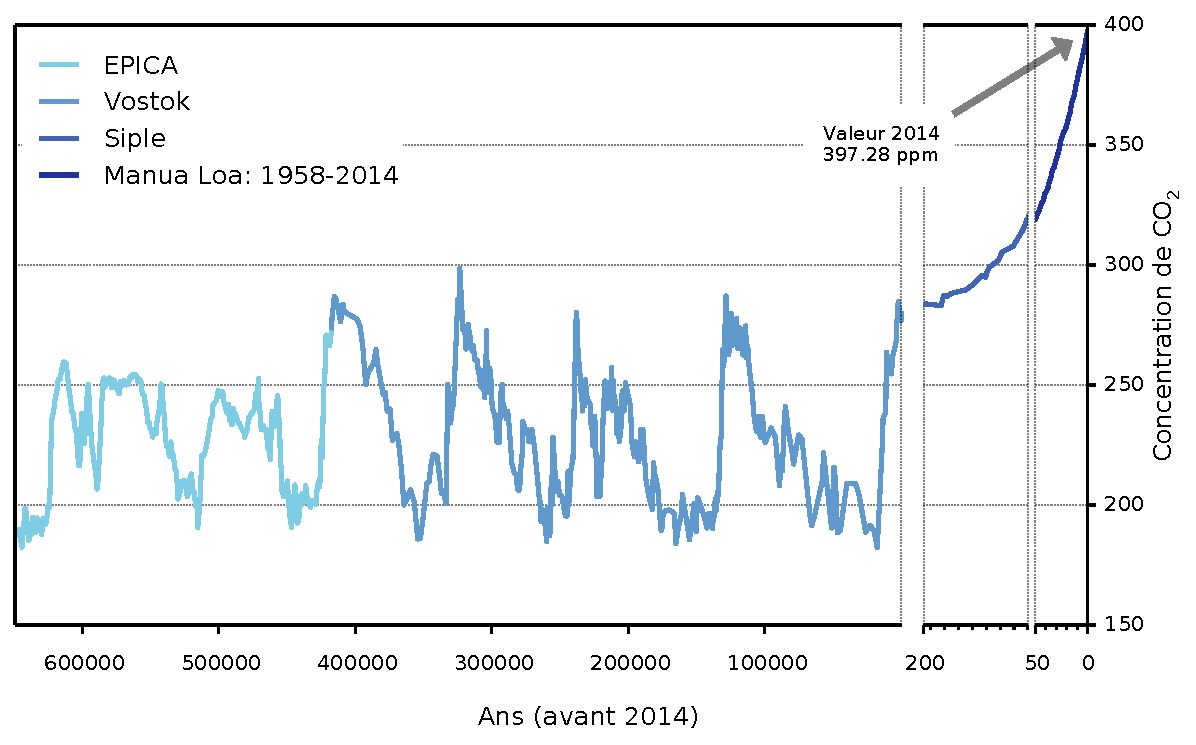
\includegraphics[width=\textwidth]{fig/CO2.pdf}
                \label{fig:CO2}
        \end{subfigure}

        \caption{Évolution des concentrations des gaz à effet de serre dans
l'atmosphère. Source des données: \citet{Epica,Siple,Vostok,WMO14} et
\url{http://www.esrl.noaa.gov/gmd/ccgg/trends}}\label{fig:GES_tot}.
\end{figure}
À partir de ces données, on peut conclure que les concentrations actuelles de
\ce{CO2} dépassent d’au moins 100 ppm le seuil d'équilibre naturel associé au
stade interglaciaire actuel. On peut aussi conclure que la concentration de
\ce{CO2} enregistrée en \num{2014} dépasse d'environ \SI{30}{\percent} les
concentrations plus élevées dans les \num{650000} dernières années. \\
Le méthane \ce{CH4} est le deuxième plus important des gaz à effet de serre. Environ
\SI{40}{\percent} des rejets de \ce{CH4} dans l'atmosphère sont d'origine
naturelle (zones humides) et \SI{60}{\percent} d'origine humaine (élevage de
bétail, riziculture, exploitation des combustibles fossiles, décharges,
combustion de biomasse) \citep{WMO2014}. Le \ce{CH4} atmosphérique a atteint un
nouveau pic en \num{2013} – \num{1824} parties par milliard (ppb) environ – en
raison de l'accroissement des émissions anthropiques. Après une période de
stabilisation, la teneur de l'atmosphère en méthane augmente de nouveau depuis
\num{2007} \citep{WMO2014}.\\
Parmi les activités humaines qui produisent des gaz à effet de serre, la
production d’énergie est de loin la plus grande source de GES et en particulier
de \ce{CO2}. La contribution de l'agriculture (qui produit principalement du
\ce{CH4} et du \ce{N2O}) et des processus industriels non reliés à la production
d'énergie est largement plus faible, comme c'est montré dans la
\cref{fig:CO2_Fossil} \citep{IEA_fossil}.
Dans l'industrie de l'énergie, le \ce{CO2} produit lors de l'utilisation des
combustibles fossiles, domine les émissions totales des GES. Personne ne peut plus nier
que la demande croissante d'énergie à partir de combustibles fossiles a un rôle
clé dans la tendance à la hausse des émissions de \ce{CO2}. Depuis la révolution
industrielle, le \ce{CO2} émis annuellement à partir des combustibles fossiles
a augmenté dramatiquement de presque \num{0} à environ \SI{32}{\giga\tonne}
\ce{CO2} en \num{2012} \citep{IEA_fossil}.\\
Dans un contexte où la demande d’énergie est de plus en plus grande, il faut
trouver des mesures permettant la mise en œuvre d'options durables en matière
de production, de distribution et de consommation finale d'énergie.
\begin{figure}[ht]
\centering
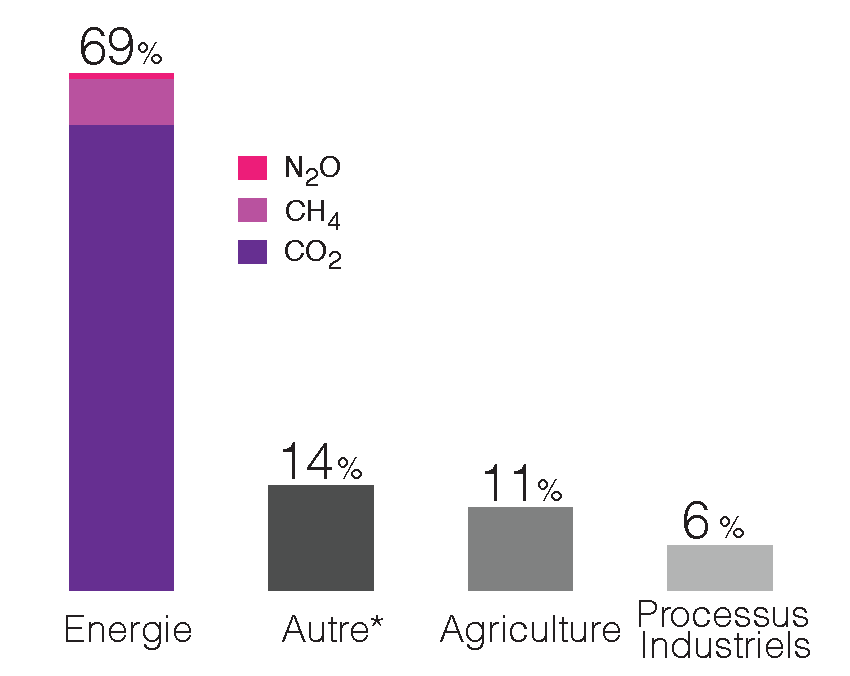
\includegraphics[width=0.7\textwidth]{fig/co2_fossil_fuel_these.pdf}
\caption{Répartitions des GES anthropiques. $^{\ast}$Autre inclut: combustion de
biomasse, émissions indirectes de \ce{N2O} non agricoles, déchets, utilisation
de solvants. Source des données: \citet{IEA_fossil}}
\label{fig:CO2_Fossil}
\end{figure}
\section{Évolution énergétique et scénario de réduction du
\texorpdfstring{\ce{CO2}}{CO2}}
L'Agence internationale de l'énergie (AIE) a publié un rapport dans lequel elle
voit une augmentation de la demande énergétique mondiale de \SI{37}{\percent}
d'ici \num{2040} \citep{WEO2014}. Bien que le choix des politiques et les
évolutions du marché devraient entraîner une baisse de la demande pour les
combustibles fossiles en \num{2040}, ceci ne suffira pas à enrayer
l'augmentation des émissions de dioxyde de carbone, ce qui provoquera une
accélération de la hausse de la température mondiale de \SI{3.6}{\degreeCelsius}
à long terme. Le (GIEC) estime que pour limiter cette hausse à
\SI{2}{\degreeCelsius}, objectif
adopté au niveau international pour prévenir les répercussions les plus graves
du changement climatique, le monde ne devra pas émettre plus de
\SI{1000}{\giga\tonne} \ce{CO2} à compter de \num{2014} \citep{WEO2014}. Les
perspectives en matière de technologies énergétiques \num{2014} \citep{ETP2014}
analysent trois voies possibles pour notre futur énergétique jusqu’en 2050. Le
scénario \SI{6}{\degreeCelsius} (6DS), qui prolonge les tendances actuelles; le
scénario \SI{4}{\degreeCelsius} (4DS), qui reflète les intentions déclarées de
certains pays de réduire les émissions de \ce{CO2} et d'encourager l’efficacité
énergétique et le scénario \SI{2}{\degreeCelsius} (2DS) qui présente un réseau
énergétique durable à faibles émissions de \ce{CO2}.
\begin{figure}[ht]
\centering
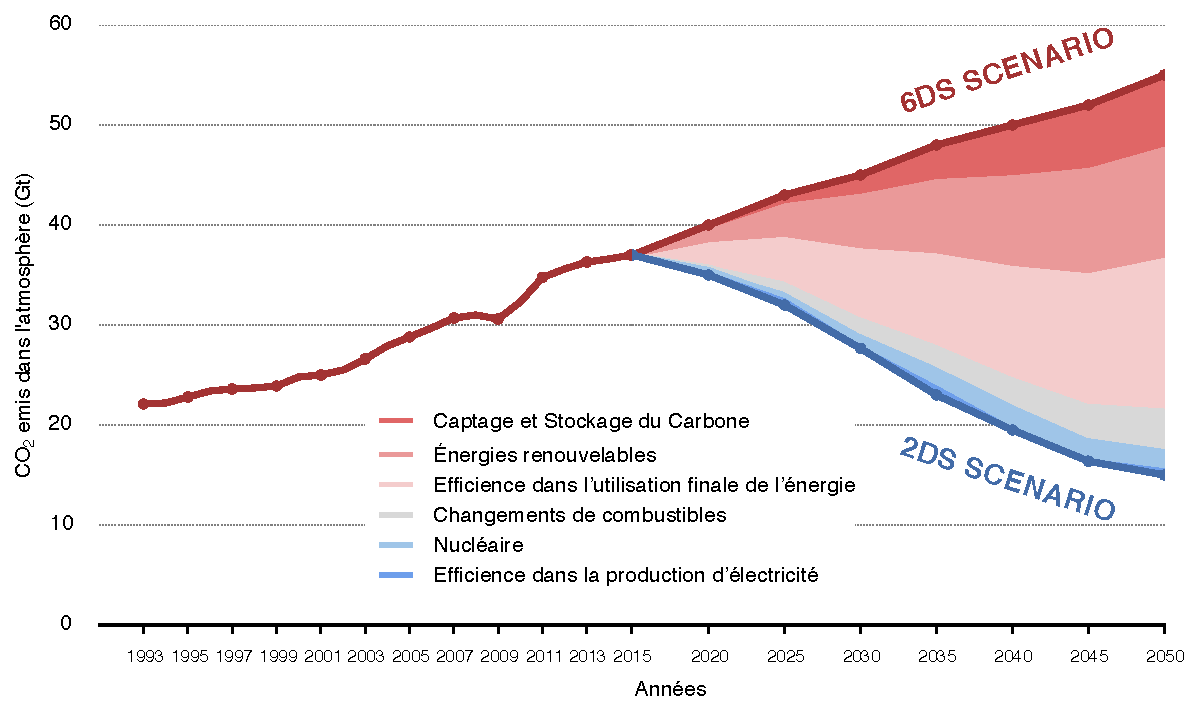
\includegraphics[width=1\textwidth]{fig/EPT2014.pdf}
\caption{Réduction des émissions du \ce{CO2} selon le type de technologie
employée. Source des données: International Energy Agency, Energy Technology
Perspectives 2014 - \url{www.iea.org/etp}}
\label{fig:ETP2014}
\end{figure}
La \cref{fig:ETP2014} montre l'évolution des émissions de \ce{CO2} globale, en
fonction du scénario suivi. Cette figure montre aussi la contribution de chaque
technologie pour atteindre le scénario 2DS, qui permettrait de limiter
l'augmentation de la température globale à \SI{2}{\degreeCelsius}.\\
Les énergies renouvelables connaissent une croissance variable et parmi elles,
l'énergie solaire, l'hydroélectricité et l'éolien terrestre sont les plus
dynamiques surtout dans les économies émergentes qui revoient leurs ambitions à
la hausse et s'affirment comme leaders du déploiement de technologies à faible
empreinte carbone \citep{ETP2014}.\\
En revanche, l'augmentation continue de la consommation de charbon contrecarre
la réduction des émissions résultant des avancées récentes du déploiement des
énergies renouvelables. Ce constat met en lumière la nécessité d'améliorer
l'efficacité des centrales à charbon et d'une utilisation à plus grande échelle
de la technologie du captage et de stockage du carbone (CSC). L'AIE et le GIEC
estiment qu’en \num{2050} environ \SI{14}{\percent} des émissions seront
réduites grâce à l'emploi du CSC. Le CSC n'est cependant pas universellement
populaire parmi les agences de protection de l’environnement et les ONG. En
effet, elle est vue comme une technologie crée par l’industrie pétrolière et
gazière qui leur permettrait de continuer à exploiter et consommer les
ressources énergétiques fossiles comme ils le font actuellement. Cependant, d'un
point de vue pragmatique, cette technologie a le potentiel de mitiger les
émissions globales durant la transition vers de nouvelles technologies à faible
empreinte carbone. Par ailleurs, il y a de nouveaux grands pollueurs comme la
Chine et l'Inde qui sont en pleine expansion économique. Les sociétés
occidentales, qui ont largement profité des énergies fossiles pour leur
développement, sont mal placées pour restreindre la consommation de ces pays.
Donc, le CSC est la seule méthode à court terme qui permettrait d'avoir un
impact significatif sur le bilan carbone.
Il faut se rendre compte que sans la
mise en place de cette technologie à grande échelle, il sera très difficile
d’atteindre les objectifs de réductions demandés par le GIEC. Il faut penser à
développer de plus en plus des projets comme celui de Boundary Dam en
Saskatchewan, où une centrale à charbon a été reconstruite avec une unité de
séquestration et stockage du \ce{CO2}. Cela permet une production
d'électricité de \SI{110}{\MW} tout en assurant une réduction des émissions de
\ce{SO2} et \ce{CO2} de presque \SI{100}{\percent} \citep{WEO2014}.\\
Comme la directrice générale de l'AIE, Maria Van der Hoeven, l'a écrit dans
l'avant-propos du rapport sur le CSC de l'AIE
\citep{IEACCS2013}:\begin{quotation} \emph{Après plusieurs années de recherche,
développements et expériences pratiques importantes, mais limitées, le temps est venu de passer à une vitesse supérieure pour le développement du CSC comme
option énergétique concrète, afin qu'il puisse être déployé à grande
échelle.}\end{quotation}
Cette citation permet de mettre en évidence l'urgence de passer des scénarios à
l'action. Étant donné les tendances passées et actuelles en matière
d’utilisation de combustibles fossiles, il y a une urgence pour le déploiement
du CSC. Cette décennie est cruciale pour faire avancer le CSC au-delà de la phase
démonstrative. Cela signifie que des actions urgentes sont nécessaires, à partir
de maintenant, de la part à la fois de l'industrie et des gouvernements pour
développer des modèles d'affaires et implémenter des cadres incitatifs qui
peuvent entraîner l'application de cette technologie dans le secteur de
l'énergie et d'autres applications industrielles. \par

Bien des gens considèrent le gaz naturel comme un combustible de transition, qui
permettrait de continuer à être dépendant aux combustibles fossiles en réduisant
les émissions de gaz à effet de serre, au cours des prochaines décennies
\citep{Pacala2004}.
Les faibles prix du gaz qui ont accompagné cette augmentation dans la production
ont mené à une croissance dans la demande de gaz. Cette croissance n'a pas été
sans controverse, en particulier dans le cas des gaz de schiste, avec les préoccupations soulevées au sujet de la pollution des
eaux \citep{Osborn2011} et les émissions des gaz à effet de serre (GES), en
particulier ceux liés à la fracturation hydraulique
\citep{Howarth2011a,Howarth2011b}.
\section{Captage et stockage du carbone (CSC)}
Le captage et le stockage du dioxyde de carbone est un processus consistant à
séparer le \ce{CO2} des autres composés industriels et énergétiques, à le
transporter dans un lieu de stockage et à l'isoler de l'atmosphère sur le long
terme \citep{IPCC2005}. Les grandes sources ponctuelles de \ce{CO2} incluent
d'importantes installations faisant appel à des combustibles fossiles (p.ex. les
raffineries et les centrales au charbon), des cimenteries ainsi que les
installations productrices de gaz naturel. Selon les GIEC et l'IEA, le stockage
géologique du \ce{CO2} (piégeage dans des couches réservoirs profondes) est la
seule
technique qui pourrait engendrer des réductions d'émissions de
\SIrange{10}{55}{\percent} à court terme. \\
La \cref{fig:ccs} montre un schéma classique de stockage géologique du
\ce{CO2}. Actuellement il y a plusieurs projets de grande envergure liés à la
séquestration géologique du \ce{CO2}. La \cref{fig:ccs_sites} montre les
principaux projets et leur capacité de stockage annuel.
\begin{figure}[ht]
\centering
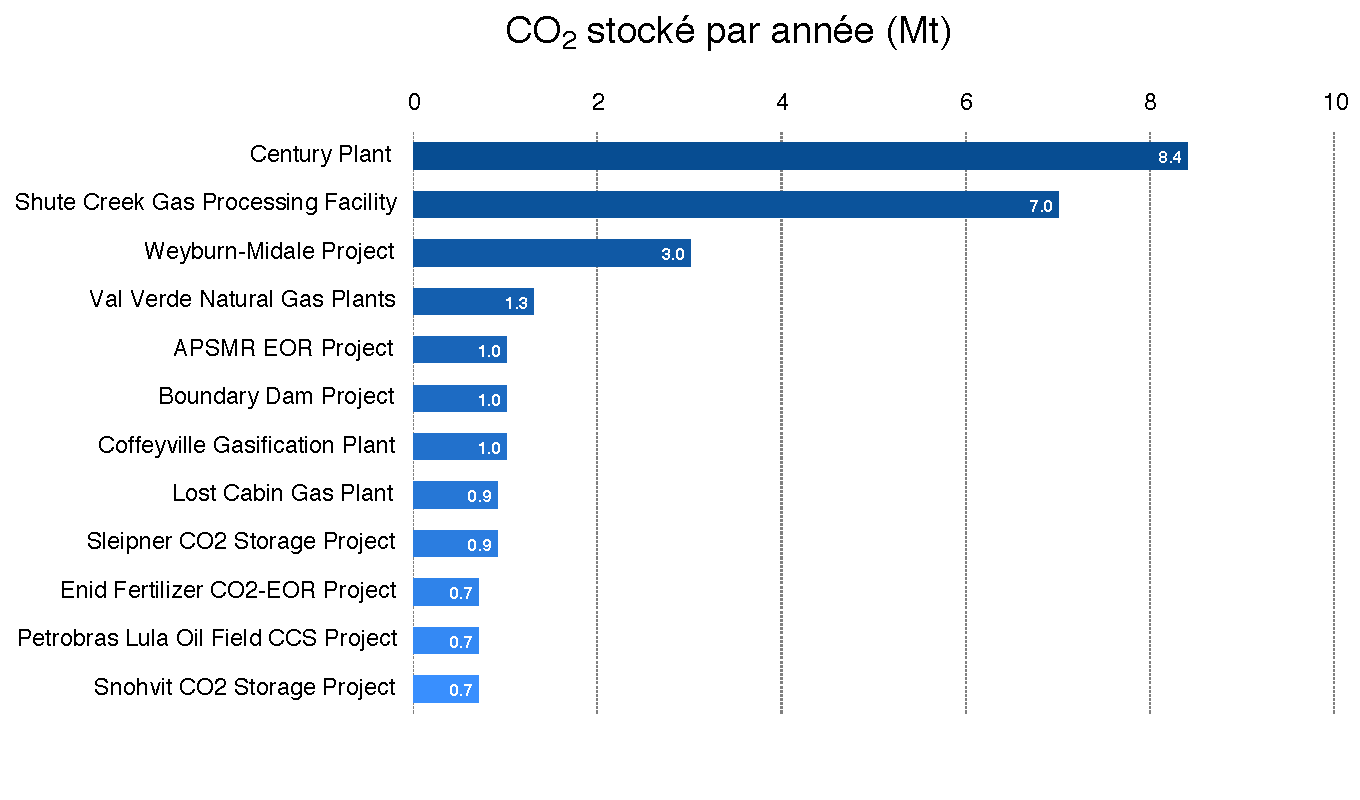
\includegraphics[width=1\textwidth]{fig/CCS_sites.pdf}
\caption{Sites CSC par volume annuel de stockage de \ce{CO2} (mis à jour de
2014). Source des données: \url{http://www.globalccsinstitute.com/}}
\label{fig:ccs_sites}
\end{figure}
Le principe de base derrière ces projets consiste à injecter du \ce{CO2}  à des
pressions d'environ \SI{8}{\mega\pascal} dans un
aquifère salin ou dans un champ de pétrole ou de gaz naturel épuisé situé à une
profondeur supérieure à \SI{800}{\metre}. À ces profondeurs, le \ce{CO2} se
trouve à l'état supercritique avec une densité d'environ
\SI{700}{\kg\per\cubic\meter} qui est plus faible que celle de la plupart des
fluides naturels (saumure ou huile) que l'on trouve dans les réservoirs. C'est
une phase aussi dense qu'un liquide, mais assurant des propriétés de transport
(viscosité et diffusion), proches de celles d'un gaz.\\
Sa flottabilité entraîne la remontée du \ce{CO2} vers la surface jusqu'à ce
qu'il rencontre une couche imperméable capable d’empêcher toute remontée
ultérieure du fluide (aussi appelée couche couverture dans le domaine
pétrolier). Ce phénomène est connu sous le nom de piégeage stratigraphique et on
estime qu’au début de l'injection, la majorité du \ce{CO2} est piégé de cette
façon \citep{Johnson2001}.\\
Par ailleurs, le \ce{CO2} en phase libre se dissout graduellement dans les
fluides résiduels
qui se trouvent dans le réservoir. La dissolution du \ce{CO2} augmente la
densité de la saumure, de sorte que la flottabilité forcera ces fluides vers le
bas en réduisant le risque de fuite. Ce phénomène est connu sous le nom de
piégeage hydrodynamique; \citet{Johnson2001} estiment que jusqu'à
\SI{15}{\percent} du \ce{CO2} peut être stocké de cette façon.\\
Le \ce{CO2} libre et la saumure enrichie de \ce{CO2} se trouvent en déséquilibre
chimique avec les roches du réservoir; des réactions chimiques qui produisent de
la dissolution ou de la précipitation auront donc lieu. Le scénario optimal est
celui où les minéraux qui contiennent des carbonates précipitent. Ce phénomène
est connu sous le nom de piégeage minéral. Cependant, le taux de précipitation
pour ce processus est très lent donc sur une échelle de temps décennale,
seulement une faible quantité (\SI{<1}{\percent}) de \ce{CO2} sera piégée de
cette façon. \citep{Johnson2001}.
\begin{figure}[ht]
\centering
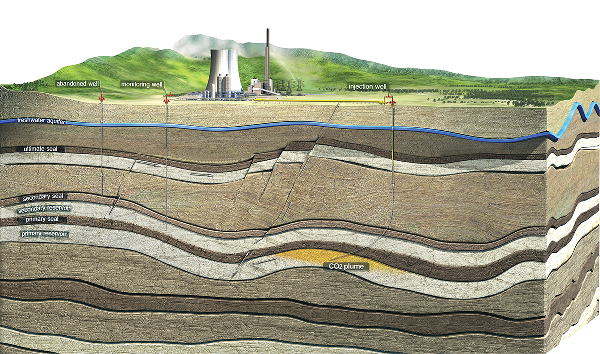
\includegraphics[width=1\textwidth]{fig/ccs.pdf}
\caption{Schéma représentant le stockage géologique du \ce{CO2}. Source de
l'image: \url{http://www.dnv.com}}
\label{fig:ccs}
\end{figure}
\subsection{Réservoirs d'hydrocarbure épuisés}
La pression des réservoirs d'hydrocarbures épuisés chute et les hydrocarbures qui étaient contenus dans les pores et les fractures
sont graduellement remplacés par les fluides de la formation, généralement de la saumure.
Depuis les années 1960, une pratique courante en ingénierie de réservoir est
celle d'injecter de la saumure pour maintenir une pression élevée. Dans certains
cas, le \ce{CO2} a été utilisé à la place de la saumure. En effet, il a été
découvert qu'en injectant du
\ce{CO2} on est capable d’augmenter l'extraction d'hydrocarbures tout en
assurant que le \ce{CO2} injecté reste en place. Ce type de stockage est
actuellement mené dans le projet de Weyburn-Midal en Saskatchewan. Il y a trois
avantages principaux à stocker le \ce{CO2} de cette façon. Premièrement, le
bénéfice économique est accru en raison d'une augmentation de l'extraction
d'hydrocarbures.
Deuxièmement, les réservoirs sont très bien étudiés et les volumes potentiels de
stockage sont connus. Finalement, la majorité des infrastructures nécessaires
sont déjà en place.\\
Cependant, il faut considérer que les puits abandonnés pourraient fournir une
voie préférentielle pour la remontée du \ce{CO2} vers la surface et que les
activités d'extraction pourraient avoir endommagé la roche couverture.
\subsection{Aquifères salins}
Le \ce{CO2} est un liquide de faible densité; il est donc piégé dans des
réservoirs poreux qui sont recouverts par une couche imperméable. Ce type de
piège stratigraphique est abondant dans la plupart des bassins sédimentaires
où les roches sont saturées en saumure. Ces aquifères salins représentent de
loin le plus grand volume disponible pour le stockage du \ce{CO2}.
\citet{Bedard2013} estiment que les aquifères salins des Basses-Terres du
St Laurent (Québec, Canada) renferment un potentiel de stockage d'environ
\SI{3}{\giga\tonne} de \ce{CO2}, ce qui représenterait les émissions de toute
la
province de Québec pendant \num{150} ans. Cependant, les aquifères salins
n'ayant aucune valeur commerciale, ils ne sont pas très bien étudiés et il est
donc
difficile d'obtenir des estimations précises ainsi que des données fiables pour
assurer la sécurité du stockage. Actuellement, il existe trois projets
importants dans ce type d'environnement, soit à Sleipner et Sn{\o}hvit, dans la
mer du Nord, et Aquistore en Saskatchewan, où la viabilité du projet de stockage
dans des aquifères
salins à été démontrée.
\section{La zone d'étude}
\label{sc:site_etude}
Le Ministère du Développement durable, de I'Environnement et des Parcs (MDDEP)
du Québec a octroyé une subvention à I'INRS-ETE pour mettre en place une chaire
de recherche sur la séquestration géologique du \ce{CO2} au Québec. Des
aquifères salins profonds ont été identifiés à plusieurs niveaux
stratigraphiques dans la région de Bécancour, entre Montréal et Québec: les
calcaires du Groupe de Trenton, les grès dolomitiques du Groupe de Beekmantown
(Formation Theresa) et les grès quartzeux du Groupe de Potsdam (Formations
Cairnside et Covey Hill). Ces aquifères sont situés à une profondeur moyenne
allant de \SIrange{795}{1230}{\metre} \citep{INRS1}. \\
Les travaux de recherche de la chaire ont montré que les épaisseurs nettes des
intervalles productifs sont plus importantes dans les grès du Groupe du Potsdam
et particulièrement dans les grès de la Formation Covey Hill (\SI{196}{\metre}).
Les grès de Covey Hill ont aussi les porosités effectives les plus importantes
(\SI{6}{\percent}), les perméabilités de la matrice les plus élevées
(\SI{2.4e-16}{\metre\squared}) ainsi qu'une salinité relativement faible
(\SI[per-mode=symbol]{108.500}{\milli\gram\per\litre}) \citep{TranNgoc2014}. Les
grès de la Formation Cairnside ont aussi un potentiel de stockage intéressant. Cependant leur faible porosité et perméabilité ainsi que leurs
eaux fortement salines sont moins favorables pour le stockage du \ce{CO2}. Les
\cref{fig:map,fig:strati} de l'\cref{ch:article1} à la \cpageref{fig:strati}
montrent les bassins sédimentaires de la zone d'études et la stratigraphie
simplifiée des Basses-Terres du St Laurent respectivement. \\
Dans ce travail, les aquifères du Groupe du Potsdam ont été choisis comme
réservoir cible pour la séquestration géologique du \ce{CO2} au Québec  pour leurs propriétes réservoirs mentionnées ci-haut. La
description des propriétés physiques des échantillons du Covey Hill et du
Cairnside sont présentés dans le \cref{tbl:prop} de l' \cref{ch:article1} à la
\cpageref{tbl:prop}.
\section{Objectifs de la thèse}
Pour que le captage et stockage du \ce{CO2} aient un impact positif sur
l'environnement, le \ce{CO2} doit donc être stocké dans le sous-sol aussi
longtemps qu'il le faut pour que les émissions anthropologiques chutent à des
niveaux acceptables et que le cycle du carbone se rétablisse et se stabilise.
Ces contraintes nécessitent que le \ce{CO2} soit stocké sur une échelle de temps
de l'ordre de \numrange{e1}{e4} ans. Pour atteindre cette exigence, on doit
s'assurer que le \ce{CO2} reste en place et ne puisse migrer sur de grandes
distances ni verticalement ni horizontalement. \\
Ceci nous oblige à répondre à deux questions scientifiques principales pour que
les projets de  CSC deviennent économiquement et politiquement acceptables:
\begin{enumerate}[-]
\item Peut-on utiliser les méthodes géophysiques pour surveiller la migration du
\ce{CO2} dans un contexte de faible porosité et perméabilité comme celui des
Basses-Terres du St Laurent?
\item Peut-on utiliser les données géophysiques afin de quantifier l'étalement
du panache de \ce{CO2} dans le sol et quantifier son incertitude?
\end{enumerate}
L'objet de cette thèse est donc d'analyser et répondre à ces questions afin de
renforcer les bases scientifiques pour le stockage du \ce{CO2} dans l'aquifère
salin des Basses-Terres du St Laurent (BTSL), identifié comme cible principale
pour le développement du CSC dans la province du Québec.
\subsection{Peut-on utiliser les méthodes géophysiques pour surveiller la
migration du \texorpdfstring{\ce{CO2}}{CO2} dans un contexte de faible
porosité et perméabilité comme celui de Basses-Terres du St Laurent?}
\label{sc:obj1}
La surveillance sismique temporelle a prouvé être une méthode
efficace pour aider à la gestion des réservoirs d'hydrocarbures depuis les
années 1990 \citep{Johnston2010}. Plus récemment, cette technique a été adoptée
à des fins de surveillance des sites de stockages de \ce{CO2} où l'objectif est
non seulement celui de surveiller le réservoir, mais aussi de sonder et
quantifier l’intégrité de la roche couverture. Cette technique a été utilisée à
Sleipner \citep{Arts2004} à Weyburn-Midale (Canada) \citep{Li2001,Davis2003,White2013} à
In Salah (Algerie) et Sn{\o}hvit (Norvège) \citep{Eiken2011} et dans le projet Aquistore (Saskatchewan) \citep{Roach2015} ainsi
que dans plusieurs projets pilotes tels que Cranfield (États-Unis) \citep{Zhang2012}, Otway (États-Unis)
\citep{Urosevic2010}, Nagaoka (Japon) \citep{Sato2011} et Ketzin (Allemagne)
\citep{Luth2011,Ivanova2012}. Dans l'ensemble, ces sites présentent des
conditions d'injection idéales avec des porosités de \SIrange[range-units =
single]{15}{20}{\percent} et des perméabilités de \SIrange[range-units =
single]{5e-12}{5e-14}{\metre\squared}.  \\
Dans le cas de la surveillance du \ce{CO2}, une des limitations majeures de la
sismique de surface, est sa résolution verticale. En effet, il est très
difficile, voire impossible, d’imager des couches plus minces que
\SIrange{10}{15}{\metre}, aux profondeurs des réservoirs ayant un potentiel de
stockage \citep{Arts2004}. Cependant, dans des environnements stratifiés, il
n'est pas rare que le \ce{CO2} reste piégé dans des couches plus minces que la
limite de résolution de la sismique de surface
\citep{Chadwick2004,Chadwick2005,Chadwick2009,Bickle2007,Lippard2008}. Le
profilage sismique vertical (PSV) pourrait partiellement résoudre le problème de
résolution. Cette méthode présente l'avantage de placer des géophones dans un
puits, au niveau du réservoir en améliorant le pouvoir de résolution. Cette
technique a été employée avec succès pour la surveillance de l'injection d'une
petite quantité de \ce{CO2} dans la Formation de Frio au Texas \citep{Daley2008}
ainsi que pour la surveillance temporelle du \ce{CO2} à Ketzin en Allemagne.
\textbf{Un des objectifs de cette thèse est donc celui de tester un modèle
numérique pour le PSV comme outil de surveillance de la propagation du \ce{CO2}
dans des conditions de très faible porosité (\SIrange[range-units =
single]{4}{6}{\percent}) et perméabilité (\SIrange[range-units =
single]{1.2e-16}{2.5e-16}{\metre\squared}).}\par

Dans les approches conventionnelles, en raison du nombre limité de puits et de
l'absence de méthode éprouvée
d'assimilation quantitative de données indirectes, les modèles géologiques
utilisés pour la modélisation sismique sont très simplistes, homogènes et ne
reflètent pas la réalité \citep{DubreuilBoisclair2012,Claprood2013}. De plus,
les algorithmes utilisés pour la propagation des ondes sismiques dans un milieu
poreux
ne tiennent pas compte de l'influence des fluides. \citet{Giroux2012} présente
une implémentation des CPML (\emph{convolutional perfectly matched layer}) pour
les milieux poroviscoélastiques isotropes et anisotropes. L'approche
poroviscoélastique est peut-être l'outil le plus efficace pour étudier l’effet
des
fluides saturant les roches, car leurs propriétés sont directement prises en
compte dans les équations. \textbf{Un autre objectif est donc de
construire un modèle géologique stochastique de référence afin de produire des
sismogrammes en utilisant une formulation poroviscoélastique. Des mesures de
laboratoires ont été nécessaires afin d’étalonner le modèle géologique.}\par

La modélisation de la réponse sismique à l'injection du \ce{CO2} nécessite des
modèles représentatifs pour prédire correctement le comportement des ondes
acoustiques traversant des milieux géologiques complexes.
Cela implique la modélisation de l'écoulement du fluide afin de prédire la
progression du panache de \ce{CO2} dans le réservoir. L'approche classique
repose sur l'utilisation des méthodes numériques en trois dimensions pour
résoudre le système avec un degré de précision élevé. Toutefois, cela implique
des efforts importants de calcul, qui ne sont pas toujours abordables ou même
possibles à mettre en oeuvre. Au cours des dernières années, des approches
employant des méthodes semi-analytiques ont été mises au point
\citep{Nordbotten2005a, Nordbotten2009}. Un outil de simulation prometteur pour
la modélisation rapide et précise de la séquestration de \ce{CO2} est basé sur
l'hypothèse d'équilibre vertical (VE). Au cours des dernières années, les
méthodes VE ont été employées pour simuler l'injection et la migration du
\ce{CO2} à grande échelle, pour laquelle l'hypothèse d'équilibre vertical avec
interface nette entre \ce{CO2} et saumure peut être formulée
\citep{Nordbotten2005a,Celia2006,Nordbotten2006}. \textbf{Finalement, le dernier
objectif de cette section est de modéliser l'injection et la migration du
\ce{CO2} avec l'hypothèse d'équilibre vertical afin de pouvoir tester le PSV
comme outils de surveillance temporelle.}
\subsection{Peut-on utiliser les données géophysiques afin de quantifier
l'étalement du panache de \texorpdfstring{\ce{CO2}}{CO2} dans le sol et
quantifier son incertitude?}
\label{sc:obj2}
Tout processus d'évaluation des ressources de stockage géologique du \ce{CO2}
nécessite des estimations de la quantité de \ce{CO2} qui peut être stockée dans
le sous-sol. Les incertitudes liées à cette estimation dépendent entre autres de
la compréhension du sous-sol en terme de données géologiques et des modèles. De
manière générale, en raison du faible nombre de données, un seul modèle
déterministe est utilisé pour évaluer la ressource d'un site de stockage du
\ce{CO2}. Cependant, étant donné que notre connaissance du sous-sol est toujours
très limitée, le modèle déterministe ne sera jamais assez fidèle à la réalité.
Finalement, on ne fournit qu'un seul modèle qui est certain d'être non réaliste
tout en négligeant l'incertitude. Cette situation peut être améliorée en
utilisant des méthodes probabilistes qui respectent l'incertitude des données
que l'on peut exploiter tant dans la construction du modèle statique (porosité,
perméabilité) que pour le suivi et l'évaluation de l'injection. De plus, dans
les cas d'injection de fluides, il est important d’intégrer la surveillance
temporelle sismique avec les simulations d’écoulement de \ce{CO2} dans un cadre
commun appelé calage historique \citep{Doyen2007}. Cette pratique est
assez bien connue dans le domaine pétrolier et gazier, mais elle n'a pas encore
été adoptée dans la séquestration et stockage du \ce{CO2}. De plus, dans le cas
de la CSC, il n'y a pas d'information directe sur le mouvement du panache, car,
dans la plupart du temps, il n'y a qu'un seul puits de surveillance.
\textbf{Un autre objectif de
la thèse est donc de définir une séquence logique de modélisation stochastique
d'un réservoir potentiel pour la séquestration géologique du \ce{CO2}. Afin de
valider l'adéquation optimale des modèles, ceux-ci sont testés en fonction de leur
réponse sismique poroviscoélastique par rapport aux données mesurées.}
